% -*- compile-command: "make HOCKING-PeakSegJoint-slides.pdf" -*-
\documentclass{beamer}
\usepackage{tikz}
\usepackage[all]{xy}
\usepackage{amsmath,amssymb}
\usepackage{hyperref}
\usepackage{graphicx}

\DeclareMathOperator*{\argmin}{arg\,min}
\DeclareMathOperator*{\Lik}{Lik}
\DeclareMathOperator*{\Peaks}{Peaks}
\DeclareMathOperator*{\Segments}{Segments}
\DeclareMathOperator*{\argmax}{arg\,max}
\DeclareMathOperator*{\maximize}{maximize}
\DeclareMathOperator*{\minimize}{minimize}
\newcommand{\sign}{\operatorname{sign}}
\newcommand{\RR}{\mathbb R}
\newcommand{\ZZ}{\mathbb Z}
\newcommand{\NN}{\mathbb N}

% Set transparency of non-highlighted sections in the table of
% contents slide.
\setbeamertemplate{section in toc shaded}[default][100]
\AtBeginSection[]
{
  \setbeamercolor{section in toc}{fg=red} 
  \setbeamercolor{section in toc shaded}{fg=black} 
  \begin{frame}
    \tableofcontents[currentsection]
  \end{frame}
}

\begin{document}

\title{PeakSegJoint: fast supervised peak detection via joint
  segmentation of count data samples}

\author{
  Toby Dylan Hocking\\
  toby.hocking@mail.mcgill.ca\\
  joint work with Guillaume Bourque}

%\date{2 April 2015}

\maketitle

\section{ChIP-seq data and previous work on peak detection}


\begin{frame}
  \frametitle{Chromatin immunoprecipitation sequencing (ChIP-seq)}
  Analysis of DNA-protein interactions.

  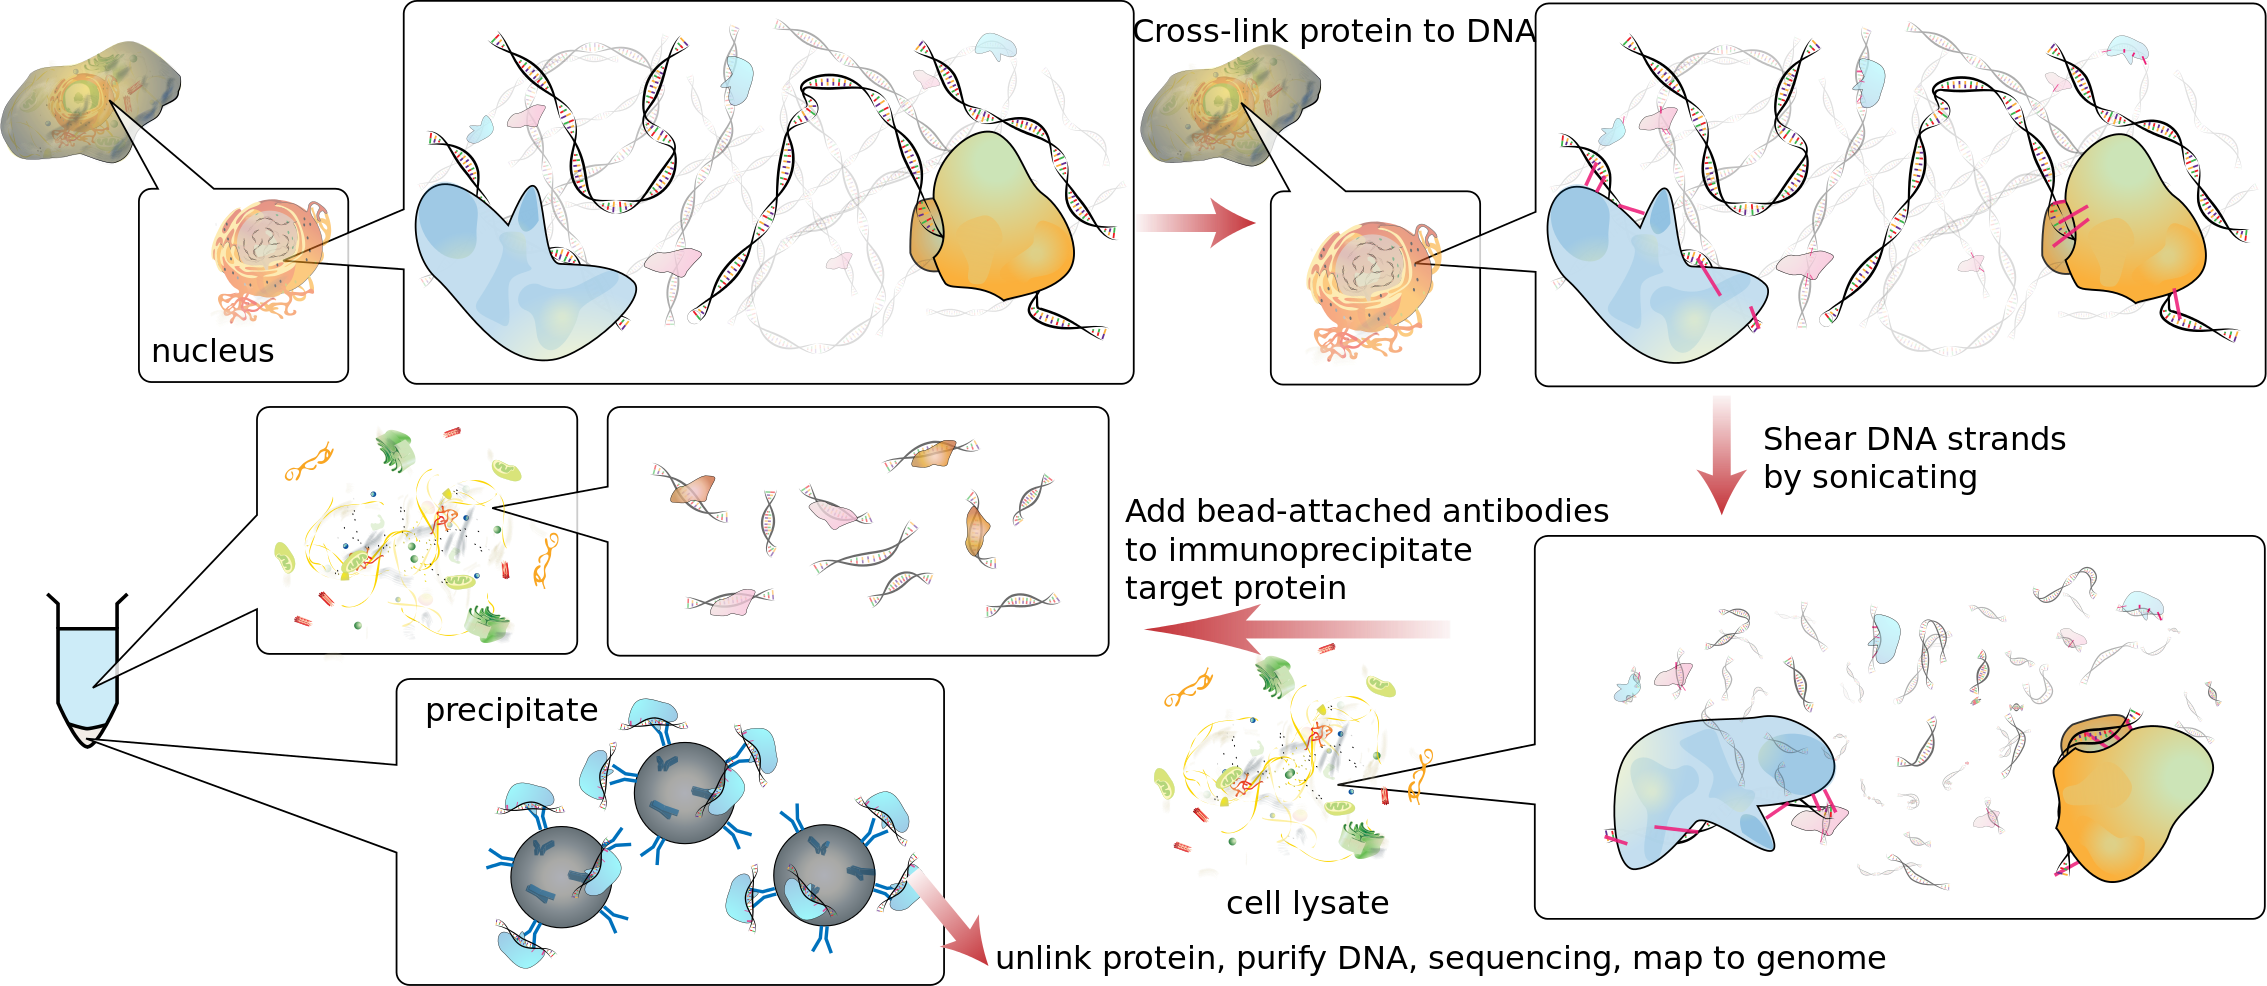
\includegraphics[width=\textwidth]{Chromatin_immunoprecipitation_sequencing_wide.png}

  Source: ``ChIP-sequencing,'' Wikipedia.
\end{frame}

\begin{frame}
  \frametitle{Problem: find peaks in each of several samples}
  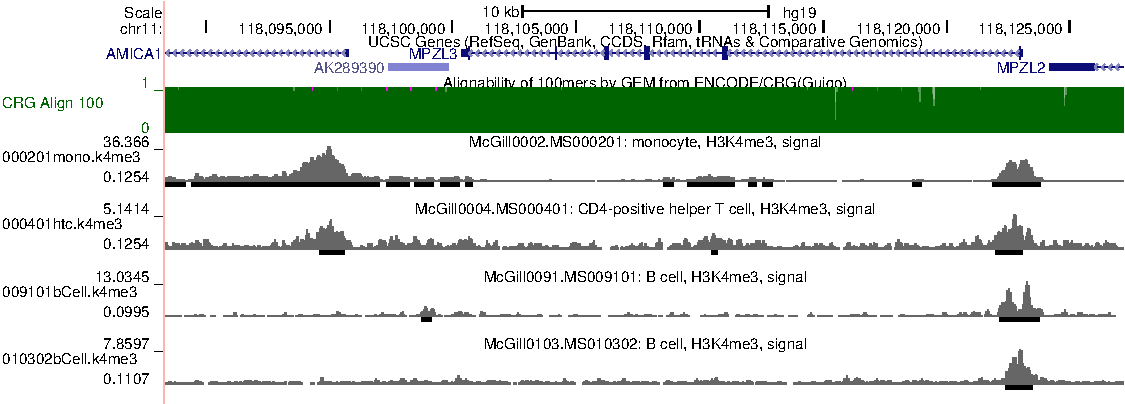
\includegraphics[width=\textwidth]{screenshot-ucsc-edited}

  Grey profiles are normalized aligned read count signals.

  Black bars are ``peaks'' called by MACS2 (Zhang et al, 2008):
  \begin{itemize}
  \item many false positives.
  \item overlapping peaks have different start/end positions.
  \end{itemize}
\end{frame}

\begin{frame}
  \frametitle{Existing peak detection algorithms}
  \begin{itemize}
  \item Model-based analysis of ChIP-Seq (MACS), Zhang et al, 2008.
  \item SICER, Zang et al, 2009.
  \item HOMER findPeaks, Heinz et al, 2010.
  \item RSEG, Song and Smith, 2011.
  \item Histone modifications in cancer (HMCan), Ashoor et al, 2013.
  \item ... dozens of others.
  \end{itemize}
  Two big questions: how to choose the best...
  \begin{itemize}
  \item ...algorithm?
  \item ...parameters?
  \end{itemize}
\end{frame}

\begin{frame}[fragile]
  \frametitle{How to choose model parameters?}
\scriptsize
19 parameters for Model-based analysis of ChIP-Seq (MACS), Zhang et al, 2008.
\begin{verbatim}
  [-g GSIZE]
  [-s TSIZE] [--bw BW] [-m MFOLD MFOLD] [--fix-bimodal]
  [--nomodel] [--extsize EXTSIZE | --shiftsize SHIFTSIZE]
  [-q QVALUE | -p PVALUE | -F FOLDENRICHMENT] [--to-large]
  [--down-sample] [--seed SEED] [--nolambda]
  [--slocal SMALLLOCAL] [--llocal LARGELOCAL]
  [--shift-control] [--half-ext] [--broad]
  [--broad-cutoff BROADCUTOFF] [--call-summits]
\end{verbatim}
10 parameters for Histone modifications in cancer (HMCan),
Ashoor et al, 2013.
\begin{verbatim}
minLength 145
medLength 150
maxLength 155
smallBinLength 50
largeBinLength 100000
pvalueThreshold 0.01
mergeDistance 200
iterationThreshold 5
finalThreshold 0
maxIter 20
\end{verbatim}
\end{frame}

\begin{frame}
  \frametitle{Previous work in computer vision: look and add labels
    to...}
  \begin{tabular}{ccc}
    Photos & Cell images & Copy number profiles \\
    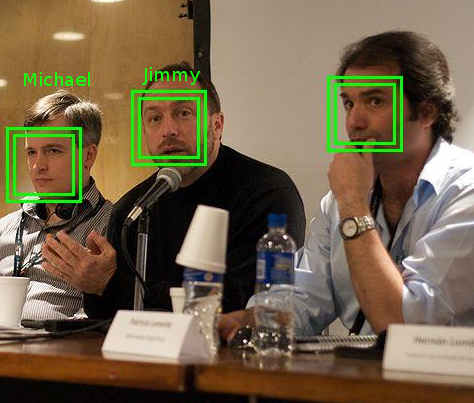
\includegraphics[width=1.3in]{faces} &
    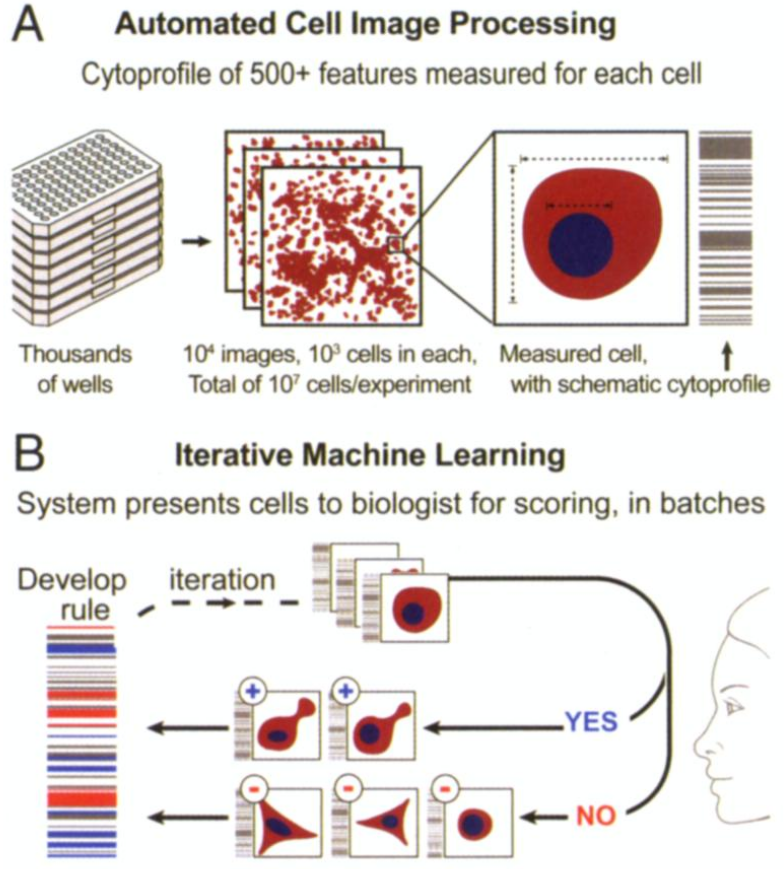
\includegraphics[width=1.3in]{cellprofiler} &
    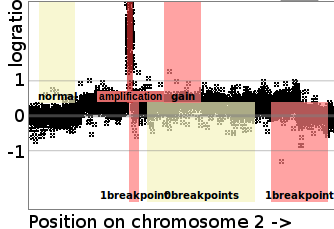
\includegraphics[width=1.5in]{regions-axes}\\
    Labels: names & phenotypes & alterations \\ \\
    CVPR 2013 & CellProfiler & SegAnnDB \\
    246 papers & 873 citations & Hocking et al, 2014. \\
     &
  \end{tabular}
  Sources: \url{http://en.wikipedia.org/wiki/Face_detection}\\
  Jones et al PNAS 2009. Scoring diverse cellular morphologies in
  image-based screens with iterative feedback and machine learning.
\end{frame}

\begin{frame}
  \frametitle{Labels indicate presence/absence of peaks}

  False negative is too few peaks, false positive is too many peaks.

  \includegraphics[width=\textwidth]{figure-good-bad}

  Goals: peaks in same positions across samples,\\
  with minimal number of incorrect regions.

\end{frame}

\begin{frame}
  \frametitle{Goal: minimize number of incorrect labels in test data}
  \begin{itemize}
  \item $S=4$ samples.
  \item $B=50,000$ base positions.
  \item $\mathbf Z \in\ZZ_+^{B\times S}$ matrix of count data.
  \item Set of labels $L$ (peaks, noPeaks, peakStart, peakEnd).
  \item Goal: find a peak caller $c:\ZZ_+^{B\times S} \rightarrow
    \{0,1\}^{B\times S}$ 
  \end{itemize}
  \begin{equation*}
    \label{eq:min_test_err}
    \minimize_c \sum_{i\in\text{test}} E[c(\mathbf Z_i),  L_i],
  \end{equation*}
  where $E$ is the number of incorrect labels\\(false positives + false
  negatives).
\end{frame}

\section{The PeakSeg and PeakSegJoint models} 

\input{figure-profiles-PeakSeg}

\begin{frame}
  \frametitle{PeakSeg single-sample model}

  \begin{itemize}
    \item Count data $\mathbf Z = \left[
    \begin{array}{ccc}
      \mathbf z_1 & \dots & \mathbf z_S
    \end{array}
    \right]\in\ZZ_+^{B\times S}$ for $S$ samples and $B$ bases.
  \item For $p\in\{0, \dots, p_{\text{max}}\}$ peaks, and for each
    sample $\mathbf z\in\ZZ_+^B$, compute the piecewise constant mean
    vector:
  \end{itemize}
  \begin{align*}
    \mathbf{\tilde m}^p(\mathbf z)  =
    \argmin_{\mathbf m\in\RR^{B}} &\ \ 
    \text{PoissonLoss}(\mathbf m, \mathbf z) 
    \\
    \text{such that} &\ \ 
    \Peaks(\mathbf m)=p,  \\
    &\ \  \alert<1>{\forall j\in\{2, \dots, B\},} 
    \ \ \alert<1>{P_j(\mathbf m) \in\{0, 1\}.}\\
    &\ \  \alert<1>{\text{up, down, up, down constraint.}}\\
    %\forall j\in\{1, \dots, B\}, &\ \ P_j(\mathbf m) \in\{0, 1\},
  \end{align*}
  \vskip -1cm
  \begin{itemize}
  \item Peak indicator: $P_j(\mathbf m) = \sum_{k=2}^j \sign( m_{k} - m_{k-1} )$.
  \item Hyper-parameters to choose: genomic window size $B$, maximum
    number of peaks $p_{\text{max}}$.
  \item $O(p_{\text{max}} B \log B)$ Constrained Dynamic Programming
    Algorithm (cDPA), Hocking et al, ICML 2015.
  \end{itemize}
\end{frame}

\input{figure-profiles}

\begin{frame}
  \frametitle{PeakSegJoint multi-sample model}
  
\end{frame}

\begin{frame}
  \frametitle{Demonstration of heuristic algorithm}

  \includegraphics[width=\textwidth]{figure-heuristic-algo}

  Interactive figure at \url{http://bit.ly/1AA6TgK}
\end{frame}

\begin{frame}
  \frametitle{H3K36me3 data, PeakSeg and Joint model}

  \includegraphics[width=1.1\textwidth]{figure-H3K36me3-profiles}

  \url{http://bl.ocks.org/tdhock/raw/b77c1a7e4d6aee40bf6c/}
\end{frame}

\section{Speed and test error results}

\begin{frame}
  \frametitle{PeakSegJoint much faster than other Poisson
    segmentation algorithms}

  Data: simulated single-sample, single-peak.

  \input{figure-timings-small} 

  pDPA from Segmentor3IsBack R package (Cleynen et al, 2014).

  cDPA from PeakSegDP R package (Hocking et al, ICML 2015).

\end{frame}

\begin{frame}
  \frametitle{Timings on example H3K36me3 data}

  \small

  Find best 0,...,9 peaks in each of 8 samples (80 PeakSeg
  models):

  \scriptsize

  \input{table-H3K36me3-PeakSeg}

  \vskip 0.2 cm

  \small

  Find best common peak in 0,...,8 samples in each of 5 genomic
  regions (45 PeakSegJoint models):

  \scriptsize

  \input{table-H3K36me3}

\end{frame}

\section{Conclusions}

\begin{frame}
  \frametitle{Thanks for your attention!}
  Write me at \alert{\texttt{toby.hocking@mail.mcgill.ca}} to collaborate!

  \vskip 1cm

  Source code for slides, figures, paper online!\\
  \small
  \url{https://github.com/tdhock/PeakSegJoint-paper}
  \vskip 1cm

  Supplementary slides appear after this one.

\end{frame}

\begin{frame}
  \frametitle{H3K27ac and Input data, PeakSeg and Joint model}

  \includegraphics[width=0.9\textwidth]{figure-H3K27ac-profiles}
\end{frame}

\begin{frame}
  \frametitle{Timings on example H3K27ac data}

  \scriptsize

  \parbox{2in}{
    Find best \\
  0,...,9 peaks\\
  in each of 8 samples\\
  (80 PeakSeg models)

  \input{table-H3K27ac-PeakSeg}
  }
  \parbox{2in}{
  Find best common peak\\
  in 0,...,8 samples\\
  in each of 11 genomic regions\\
  (99 PeakSegJoint models)

  \input{table-H3K27ac}
  }

\end{frame}

\begin{frame}
  \frametitle{H3K4me3 data, PeakSeg and Joint model}

  \includegraphics[width=\textwidth]{figure-H3K4me3-profiles}
\end{frame}

\begin{frame}
  \frametitle{Timings on example H3K4me3 data}

  \small

\parbox{1.5in}{
  Find best \\
  0,...,9 peaks\\
  in each of 10 samples\\
  (100 PeakSeg models)

  \input{table-H3K4me3-PeakSeg}
}
\parbox{2in}{
  Find best common peak\\
  in 0,...,10 samples\\
  in each of 10 genomic regions\\
  (110 PeakSegJoint models)

  \input{table-H3K4me3}
}

\end{frame}

\begin{frame}
  \frametitle{NRSF transcription factor data, PeakSeg and Joint model}

  \includegraphics[width=\textwidth]{figure-nrsf-profiles}
\end{frame}

\begin{frame}
  \frametitle{Timings on example transcription factor data}

  \scriptsize

  Find best \\
  0,...,9 peaks\\
  in each of 4 samples\\
  (40 PeakSeg models)

  \input{table-nrsf-PeakSeg}

  \vskip 0.2cm

  Find best common peak\\
  in 0,...,4 samples\\
  in each of 5 genomic regions\\
  (25 PeakSegJoint models)

  \input{table-nrsf}

\end{frame}

\begin{frame}
  \frametitle{Bin factor parameter controls optimality and speed}
  \includegraphics[width=\textwidth]{figure-bin-factor}

  H3K36me3 example data set, PeakSegJoint model with 2 peaks.
\end{frame}

\begin{frame}
  \frametitle{H3K36me3 data, cDPA and heuristic algorithms}

  \includegraphics[width=\textwidth]{figure-heuristic-profiles}
\end{frame}

\begin{frame}
  \frametitle{Heuristic is much faster than cDPA}

  \includegraphics[height=0.9\textheight]{figure-heuristic-times}
\end{frame}

\begin{frame}
  \frametitle{Heuristic often as good as cDPA}

  \includegraphics[height=0.9\textheight]{figure-heuristic-loss}
\end{frame}


\begin{frame}
  \frametitle{Weighted train error not good for model selection}

  \includegraphics[height=0.9\textheight]{figure-weighted-error}
\end{frame}

\begin{frame}
  \frametitle{Select L1-regularized model with minimal validation error}

  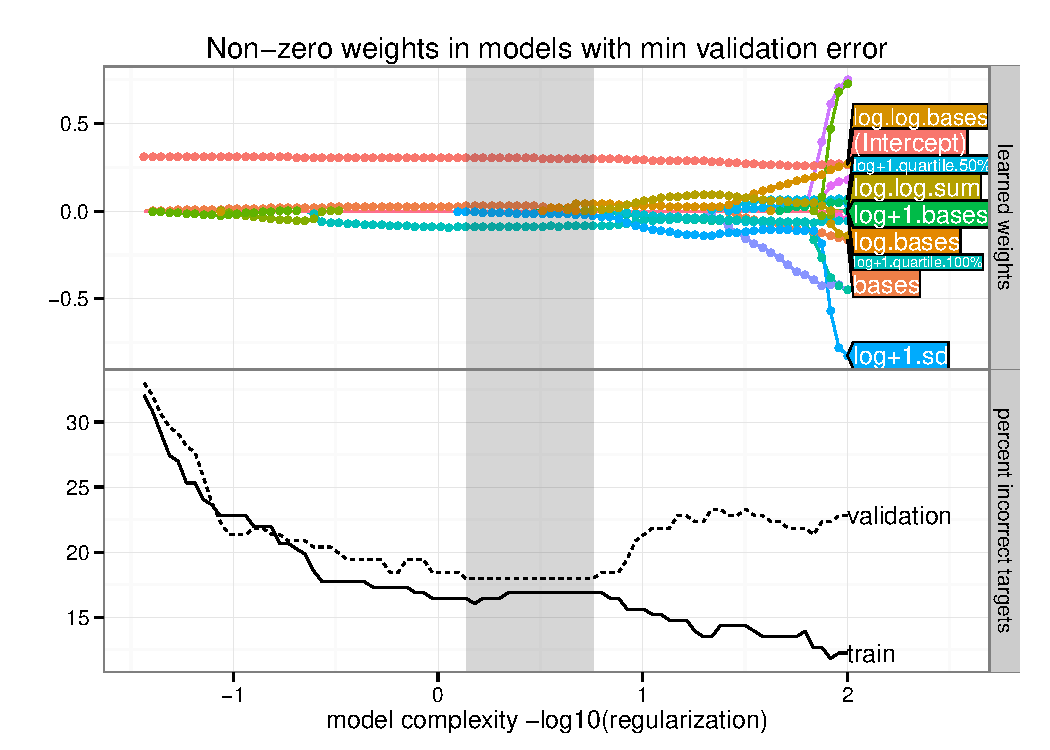
\includegraphics[height=0.9\textheight]{figure-lasso-path}
\end{frame}

\end{document}
